\section{Quantitative Results}
\label{sec:results}

\subsection{Main comparison}

\begin{table}[H]
\centering\footnotesize
\setlength{\tabcolsep}{3.5pt}
\caption{Main results ($N=10{,}000$ samples against the CIFAR-10 training set). $\pm$: standard deviation over three
independent sample sets (evaluation noise). NFE: network evaluations per image. Bits/dim: test-set bound; it is a
property of the model, so both DDPM rows share it.}
\label{tab:main}
\resizebox{\textwidth}{!}{%
\begin{tabular}{@{}lccccccrr@{}}
\toprule
Model & FID$\downarrow$ & IS$\uparrow$ & KID$\times10^3\!\downarrow$ & Prec.$\uparrow$ & Rec.$\uparrow$ & Bits/dim$\downarrow$ & NFE & Img/s$\uparrow$\\
\midrule
\textit{Real test images} & \textit{3.15} & \textit{10.97} & \textit{$-$0.01} & \textit{0.681} & \textit{0.693} & -- & -- & --\\
VAE-MLP & 135.97\,$\pm$\,0.52 & 3.11\,$\pm$\,0.02 & 127.57\,$\pm$\,0.62 & 0.323\,$\pm$\,0.006 & 0.003\,$\pm$\,0.001 & 6.313 & 1 & 350{,}102\\
VAE-Conv & 121.85\,$\pm$\,0.30 & 3.88\,$\pm$\,0.05 & 151.18\,$\pm$\,0.45 & 0.404\,$\pm$\,0.010 & 0.073\,$\pm$\,0.020 & 5.826 & 1 & 7{,}017\\
\textbf{DDPM}, 1000 steps & \textbf{6.58} & \textbf{8.59} & \textbf{1.54} & \textbf{0.694} & 0.583 & \textbf{3.794} & 1000 & 4.2\\
DDPM, DDIM 100 steps & 9.66\,$\pm$\,0.06 & 8.31\,$\pm$\,0.10 & 6.35\,$\pm$\,0.14 & 0.641\,$\pm$\,0.007 & \textbf{0.592}\,$\pm$\,0.008 & 3.794 & 100 & 41.6\\
\bottomrule
\end{tabular}}
\end{table}

\begin{itemize}
  \item \textbf{The DDPM wins every quality metric by a wide margin.} Its FID is $18.5\times$ lower than VAE-Conv's
        and its IS $2.2\times$ higher. Its precision ($0.694$) equals that of real images ($0.681$), and its recall
        is $8\times$ VAE-Conv's.
  \item \textbf{The VAE is about $1{,}700\times$ faster} ($7{,}017$ vs.\ $4.2$ images/s; $14$\,ms vs.\ $21.8$\,s for a
        single image).
  \item \textbf{Between the two VAEs,} the convolutional network is better on FID, IS, precision, recall and
        likelihood, but worse on KID. Both VAEs are far from the data distribution, where the metrics stop ranking
        models consistently, so we conclude only that VAE-Conv is better on most measures.
\end{itemize}

\paragraph{Comparison with the original paper.}
\begin{itemize}
  \item \textbf{Likelihood.} After $150$k of the paper's $800$k steps, our DDPM's test bound is $3.794$\,bits/dim
        with $\sigma_t^2=\beta_t$, or $3.781$ with $\sigma_t^2=\btil_t$. The paper reports $\le3.75$ for
        $L_\text{simple}$ (\citealp{ho2020ddpm}, Table~2). Agreement to within $0.04$\,bits/dim is strong evidence
        that the network, schedule and bound are implemented correctly.
  \item \textbf{FID and IS.} The paper reports $3.17$ and $9.46$ with $50$k samples and its best checkpoint. Our
        $6.58$ and $8.59$ use $10$k samples (which raises FID) and the final checkpoint. Training was also $5.3\times$
        shorter, and FID was still falling at the end of training (\cref{fig:fid-train}).
\end{itemize}

\subsection{Speed--quality trade-off}

\begin{figure}[H]
\centering
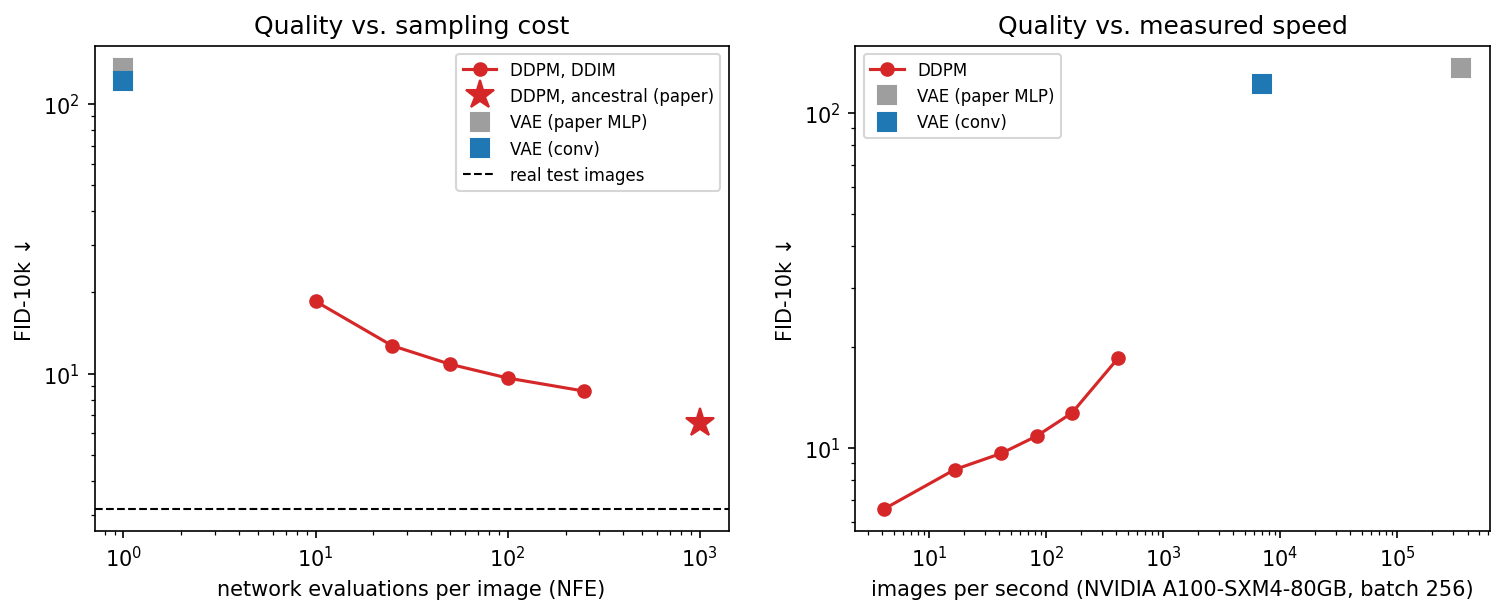
\includegraphics[width=\textwidth]{fig_speed_quality.png}
\caption{Left: FID against the number of network evaluations per image (log--log). Right: FID against measured
throughput. DDIM traces a frontier with the \emph{same} trained DDPM; the VAEs are single points at one
evaluation.}
\label{fig:speed}
\end{figure}

\begin{table}[H]
\centering\small
\caption{DDPM sampling steps (same network; DDIM sets share their starting noise).}
\label{tab:ddim}
\begin{tabular}{@{}lrcccccr@{}}
\toprule
Sampler & NFE & FID$\downarrow$ & IS$\uparrow$ & Precision & Recall & Img/s & Latency (1 image)\\
\midrule
Ancestral (paper) & 1000 & \textbf{6.58} & \textbf{8.59} & \textbf{0.694} & 0.583 & 4.2 & 21.75\,s\\
DDIM & 250 & 8.61 & 8.36 & 0.643 & \textbf{0.595} & 16.6 & 5.41\,s\\
DDIM & 100 & 9.63 & 8.24 & 0.639 & 0.584 & 41.6 & 2.20\,s\\
DDIM & 50 & 10.84 & 8.11 & 0.632 & 0.572 & 83.3 & 1.12\,s\\
DDIM & 25 & 12.70 & 8.02 & 0.626 & 0.555 & 166.5 & 0.55\,s\\
DDIM & 10 & 18.55 & 7.72 & 0.595 & 0.509 & 415.6 & 0.23\,s\\
\midrule
\textit{VAE-Conv} & \textit{1} & \textit{121.85} & \textit{3.88} & \textit{0.404} & \textit{0.073} & \textit{7{,}017} & \textit{14\,ms}\\
\bottomrule
\end{tabular}
\end{table}

\begin{itemize}
  \item DDIM with 10 steps is $100\times$ faster than the paper's sampler and still $6.6\times$ better in FID than
        VAE-Conv.
  \item DDIM does not reach the ancestral sampler's quality even at 250 steps.
  \item No DDPM setting matches the VAE's speed: at 10 steps it is still $17\times$ slower.
\end{itemize}

\subsection{Quality versus diversity}

\begin{figure}[H]
\centering
\begin{minipage}[c]{0.48\textwidth}
\centering
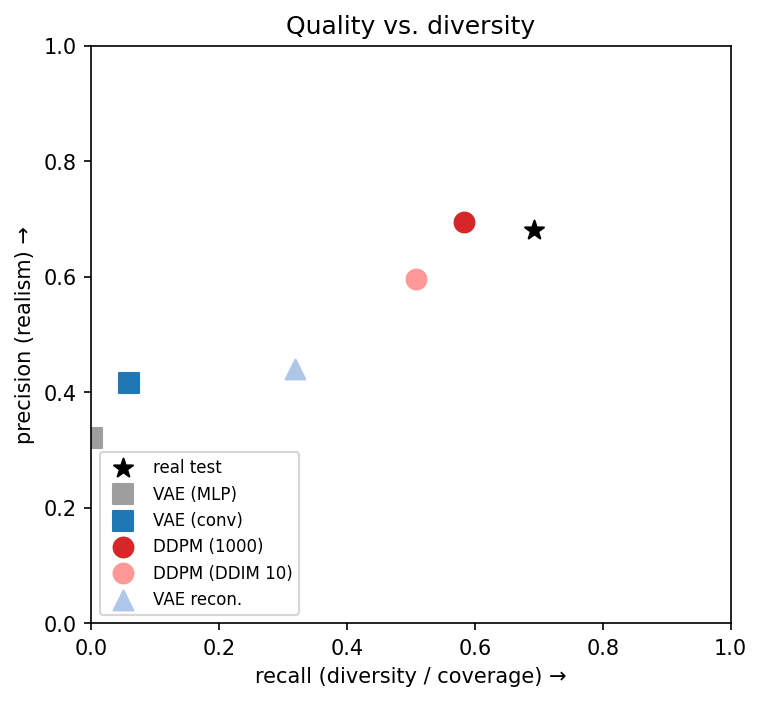
\includegraphics[width=\textwidth]{fig_precision_recall.png}
\end{minipage}\hfill
\begin{minipage}[c]{0.48\textwidth}
\caption{Precision (realism) against recall (diversity), both computed in Inception feature space. Real test
images (star) mark the ceiling. The DDPM sits next to them; both VAEs are in the low-recall corner. VAE-Conv's
reconstructions (triangle) cover far more of the data than its samples do.}
\label{fig:pr}
\end{minipage}
\end{figure}

\begin{figure}[H]
\centering
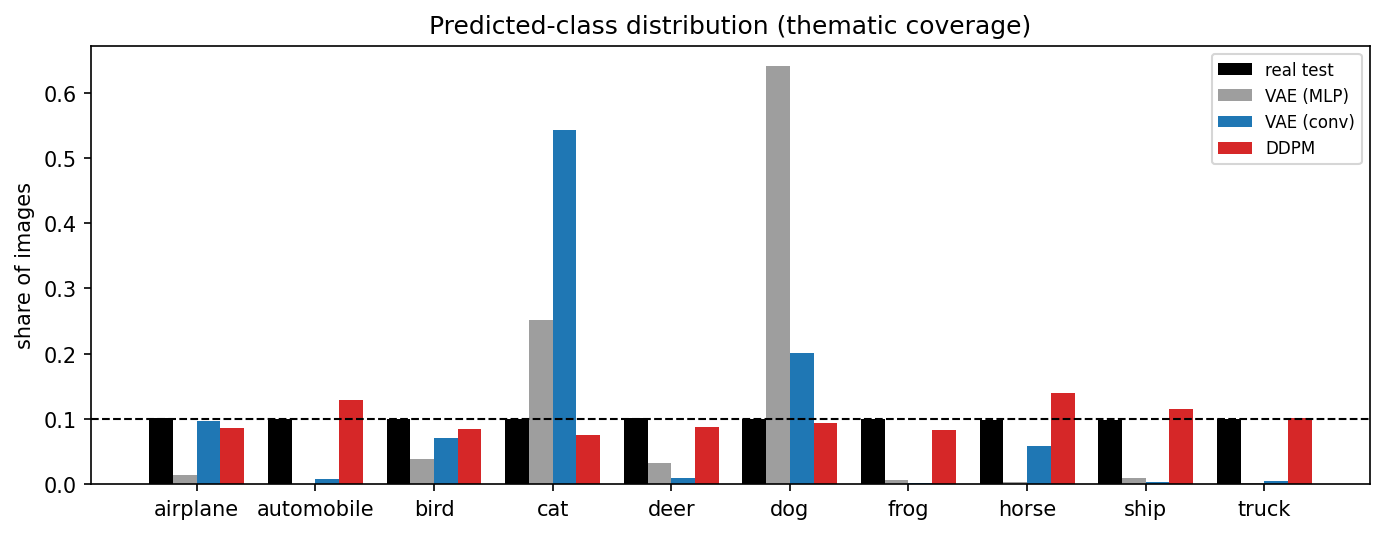
\includegraphics[width=0.92\textwidth]{fig_class_distribution.png}
\caption{Distribution of the classes predicted by the CIFAR-10 classifier for each model's samples. Dashed line:
the uniform share of $0.1$ that real data has.}
\label{fig:classes}
\end{figure}

The DDPM lies next to the real-data point in \cref{fig:pr}, while both VAEs sit in the low-recall corner. The VAEs'
main failure is therefore \emph{coverage}, not only blur. VAE-Conv's \emph{reconstructions} reach a recall of
$0.32$, which points to the cause (\cref{sec:prior-hole}).

\begin{table}[H]
\centering\small
\caption{Thematic consistency, measured by a CIFAR-10 classifier (93.6\% accuracy on real test images).}
\label{tab:thematic}
\begin{tabular}{@{}lcccc@{}}
\toprule
Images & Mean conf.$\uparrow$ & Conf.\ $>0.9\uparrow$ & Class entropy (1 = even) & Rarest class share\\
\midrule
Real test images & 0.875 & 0.742 & 1.000 & 0.098\\
VAE-MLP & 0.756 & 0.298 & 0.455 & 0.000\\
VAE-Conv & 0.692 & 0.164 & 0.601 & 0.003\\
DDPM (1000 steps) & \textbf{0.865} & \textbf{0.719} & \textbf{0.991} & \textbf{0.076}\\
DDPM (DDIM 100) & 0.854 & 0.670 & 0.995 & 0.080\\
\bottomrule
\end{tabular}
\end{table}

\begin{itemize}
  \item \textbf{DDPM samples are almost as recognisable as real photographs} (confidence 0.865 vs.\ 0.875), and all
        ten classes appear in nearly equal shares.
  \item \textbf{The VAEs' class distribution collapses.} The classifier labels $54\%$ of VAE-Conv samples ``cat''
        and $64\%$ of VAE-MLP samples ``dog'', while automobile, frog, ship and truck almost vanish from VAE-Conv's
        samples.
  \item \textbf{This does not mean the VAE ``draws cats''.} Its blurry, brownish samples fall \emph{between}
        classes, and an uncertain classifier assigns them to broad animal classes. Only $16\%$ of VAE-Conv samples
        are classified with confidence above $0.9$, against $72\%$ for the DDPM.
\end{itemize}

\subsection{Training dynamics and the VAE's prior hole}
\label{sec:prior-hole}

\begin{figure}[H]
\centering
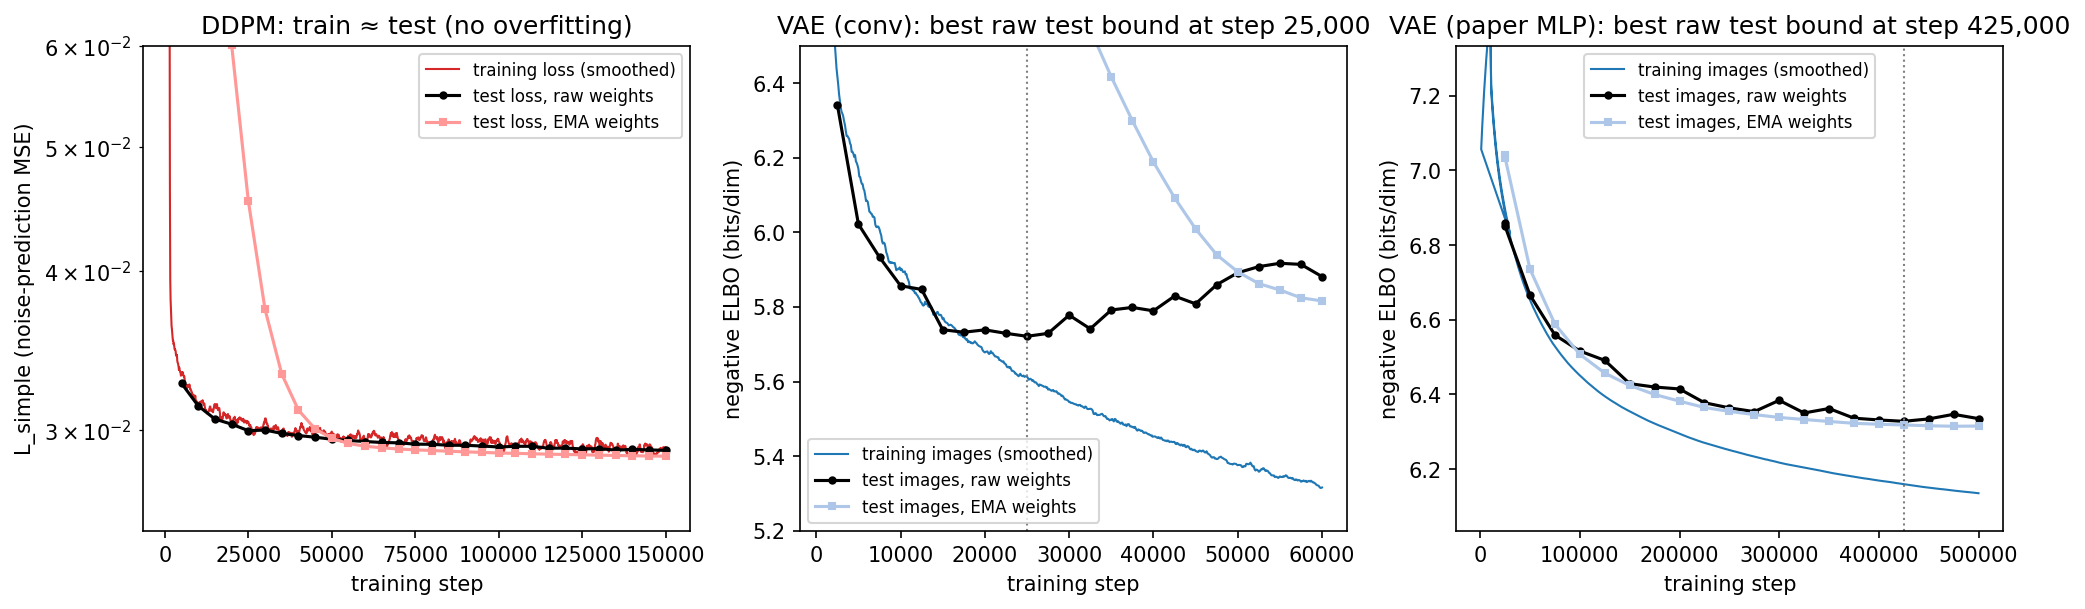
\includegraphics[width=\textwidth]{fig_training_curves.png}
\caption{Training and test objectives. DDPM: training and test losses coincide, so there is no overfitting.
VAE-Conv: the test bound is best at step 25k and then rises while the training bound keeps falling. VAE-MLP
overfits only slightly.}
\label{fig:curves}
\end{figure}

\begin{itemize}
  \item \textbf{VAE-Conv overfits its likelihood.} Its best test bound was $5.72$\,bits/dim at step $25$k. By
        step $60$k the training bound had fallen to $5.32$ while the raw-weight test bound had risen to $5.88$;
        the EMA weights we evaluate reach $5.82$.
  \item \textbf{VAE-MLP overfits only slightly:} $6.14$\,bits/dim on training images vs.\ $6.32$ on test images at
        the end of training.
  \item \textbf{The DDPM does not overfit.} Its final test loss ($0.0289$) matches its training loss ($0.0292$).
        Its EMA weights start far worse than the raw weights because, as in the paper, the EMA (decay $0.9999$) has
        no warm-up and still contains much of the random initialisation early on. They catch up after about 45k
        steps.
\end{itemize}

\begin{figure}[H]
\centering
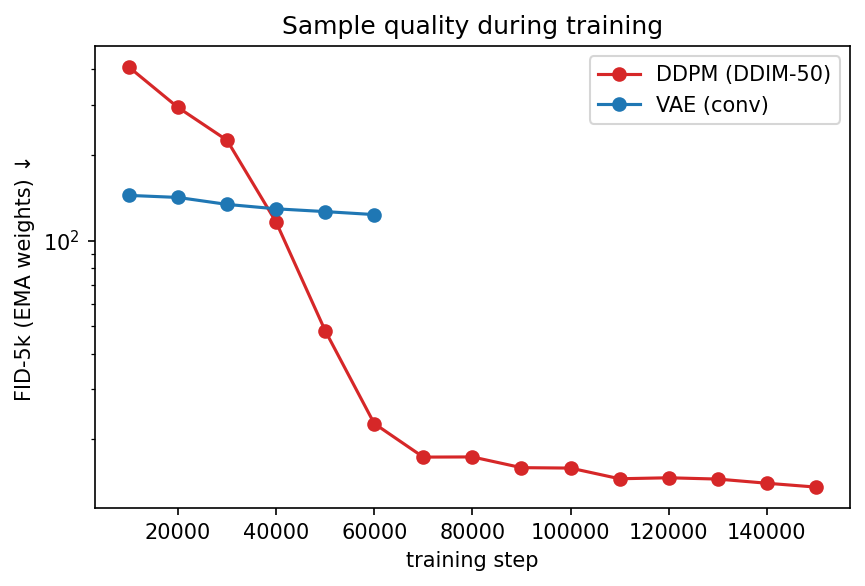
\includegraphics[width=0.62\textwidth]{fig_fid_during_training.png}
\caption{FID during training (5k samples, EMA weights; DDPM sampled with DDIM-50). The DDPM's FID keeps improving
long after its loss has flattened, and was still falling at 150k steps.}
\label{fig:fid-train}
\end{figure}

\paragraph{Likelihood and sample quality disagree.}
\begin{itemize}
  \item VAE-Conv's FID kept improving (144 $\to$ 123) while its test likelihood got worse.
  \item The DDPM's loss was flat from about 20k steps, while its FID fell from $408$ (10k steps) to $22.7$ (60k)
        and $13.6$ (150k).
\end{itemize}
This illustrates the observation of \citet{theis2016note} that likelihood and sample quality are distinct
objectives.

\paragraph{The prior hole, measured.}
\begin{itemize}
  \item VAE-Conv's \emph{reconstructions} of test images reach FID $57.9$ and recall $0.32$.
  \item Its \emph{samples} from $p(\z)$ reach FID $121.9$ and recall $0.07$.
\end{itemize}
The decoder can produce far better images than it does when sampling from the prior. The reason is that the
aggregate posterior $q_\phi(\z)=\E_{\x}\,q_\phi(\z\mid\x)$ does not fill $\N(\mathbf{0},\I)$, so a random
$\z\sim\N(\mathbf{0},\I)$ often lands where the decoder never received training signal. This is not posterior
collapse: all $128$ latent dimensions are active~\citep{burda2016iwae}, with a KL of $381$\,nats. The DDPM avoids
the problem by construction: its prior term $L_T$ is $8\times10^{-6}$\,bits/dim.

\subsection{Likelihood decomposition}

\begin{figure}[H]
\centering
\begin{minipage}[c]{0.5\textwidth}
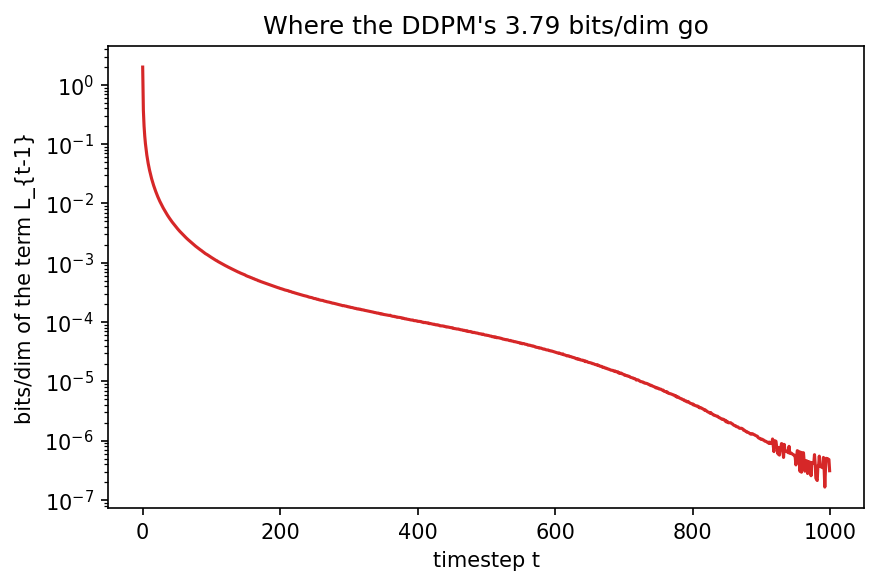
\includegraphics[width=\textwidth]{fig_bits_per_timestep.png}
\end{minipage}\hfill
\begin{minipage}[c]{0.46\textwidth}
\small
\begin{tabular}{@{}lc@{}}
\toprule
Model & Test bits/dim$\downarrow$\\
\midrule
VAE-MLP (ELBO) & $6.313\pm0.006$\\
VAE-Conv (ELBO) & $5.826\pm0.007$\\
DDPM, $\sigma_t^2=\beta_t$ & $3.794\pm0.015$\\
DDPM, $\sigma_t^2=\btil_t$ & $3.781\pm0.019$\\
\bottomrule
\end{tabular}\\[4pt]
\footnotesize $\pm$: standard error. DDPM: 1,000 test images (1000 network evaluations each); VAEs: all 10,000.
\end{minipage}
\caption{Left: contribution of each term $L_{t-1}$ of \cref{eq:vlb} to the DDPM's $3.79$\,bits/dim. Right: test
likelihood bounds of all models.}
\label{fig:bpd}
\end{figure}

Of the DDPM's $3.79$\,bits/dim:
\begin{itemize}
  \item $1.99$ ($52\%$) are spent on the final decoder term $L_0$;
  \item $3.57$ ($94\%$) are spent on the last 50 of the 1000 steps;
  \item the first $\sim\!900$ steps, where the content of the image is decided (\cref{sec:qualitative}), cost
        almost nothing.
\end{itemize}
Most of the code length therefore describes imperceptible detail, which explains how a model can have excellent
samples without a state-of-the-art likelihood. This matches the interpretation in Section~4.3 of
\citet{ho2020ddpm}. For comparison, VAE-Conv spends $0.18$\,bits/dim ($381$\,nats per image) on the KL term that
keeps its posterior close to the prior, while the DDPM's prior term $L_T$ is negligible.

\subsection{Ablations without extra training, and memorisation}

\begin{table}[H]
\centering\small
\caption{Left: effect of EMA weights (DDIM-100 for the DDPM). Right: memorisation check, i.e.\ nearest-neighbour
distance to the training set relative to unseen real test images, and the share of samples closer than the real
test images' 1st percentile (a copying model would score $\gg0.01$).}
\label{tab:ablations}
\begin{minipage}[t]{0.55\textwidth}
\centering
\begin{tabular}{@{}lcccc@{}}
\toprule
 & FID$\downarrow$ & IS & Prec. & Rec.\\
\midrule
DDPM, EMA & \textbf{9.63} & \textbf{8.24} & \textbf{0.639} & 0.584\\
DDPM, raw & 19.50 & 7.53 & 0.568 & \textbf{0.608}\\
VAE-Conv, EMA & 121.51 & 3.87 & 0.415 & 0.059\\
VAE-Conv, raw & \textbf{118.90} & \textbf{3.90} & 0.412 & \textbf{0.076}\\
\bottomrule
\end{tabular}
\end{minipage}\hfill
\begin{minipage}[t]{0.42\textwidth}
\centering
\begin{tabular}{@{}lcc@{}}
\toprule
 & NN ratio & $<$ 1st pct.\\
\midrule
VAE-MLP & 1.302 & 0.0000\\
VAE-Conv & 1.337 & 0.0000\\
DDPM & 1.024 & 0.0009\\
\bottomrule
\end{tabular}
\end{minipage}
\end{table}

\begin{itemize}
  \item \textbf{EMA halves the DDPM's FID.} For VAE-Conv it slightly \emph{hurts} FID, by more than the evaluation
        noise, although it gives the better test likelihood. This is one more instance of likelihood and sample
        quality disagreeing.
  \item \textbf{No memorisation.} DDPM samples are about as close to the training set as unseen real images are,
        and only $0.09\%$ are unusually close. \Cref{fig:nn} shows the DDPM's eight closest samples: they share pose
        and subject with their nearest training images but differ in colour, background and detail. The VAE's
        samples are far from every training image because they are blurry.
\end{itemize}

\begin{figure}[H]
\centering
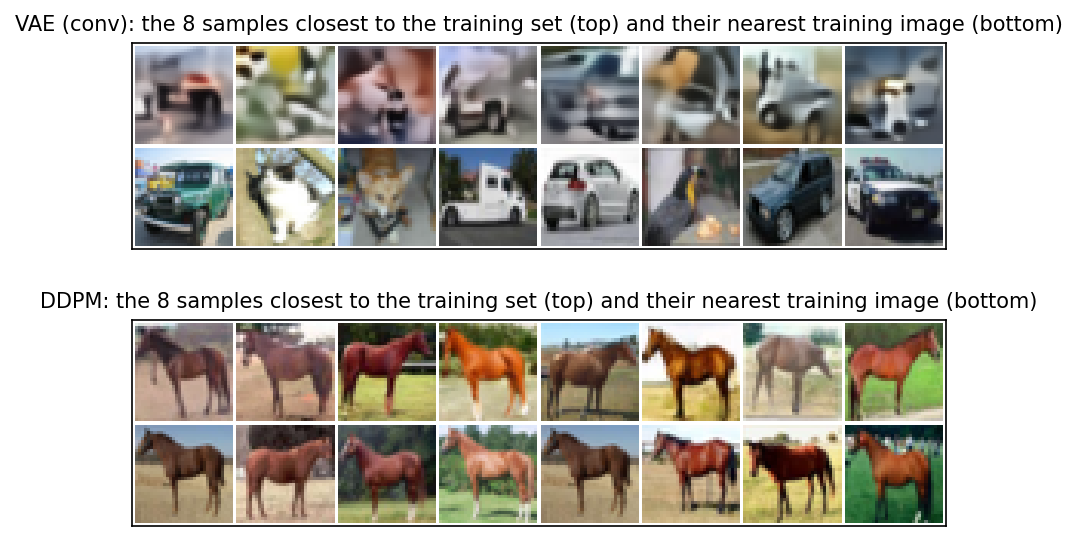
\includegraphics[width=0.8\textwidth]{fig_nearest_neighbours.png}
\caption{The eight samples closest to the training set (top row of each pair) and their nearest training images
(bottom row), in Inception feature space. Even the closest DDPM samples are new images, not copies.}
\label{fig:nn}
\end{figure}
